\documentclass[10pt]{article}
\usepackage[margin=0.55in]{geometry}
\usepackage{amsmath, amssymb}
\usepackage{enumitem}
\usepackage{titlesec}
\usepackage{tikz}
\usetikzlibrary{patterns, arrows.meta}
\usepackage{wrapfig}
\setlist{nosep, leftmargin=1.2em}
\titlespacing*{\section}{0pt}{5pt}{2pt}
\titleformat{\section}{\normalsize\bfseries}{}{0pt}{}
\setlength{\parskip}{3pt}
\setlength{\parindent}{0pt}
\pagestyle{empty}

\begin{document}

\begin{center}{\large\bfseries Perfect Punching --- Plate FEA White Paper}\end{center}

\section*{What the solver does}
Given a slab polygon, a set of columns with footprint $c_1\!\times\! c_2$, and optional walls, the solver recovers per-column shear $V_u$ and unbalanced moments $M_{u,2},\,M_{u,3}$ for the punching check. The slab is modeled as a Kirchhoff thin plate discretized with \textbf{DKT} triangles (three DOFs per node: deflection $w$ and rotations $\theta_x,\theta_y$). Material is linear-elastic isotropic concrete with $E = 57\,000\sqrt{f'_c}$ psi and $\nu = 0.2$.

\section*{Mesh}

\begin{wrapfigure}{r}{0.40\textwidth}
\vspace{-10pt}
\centering
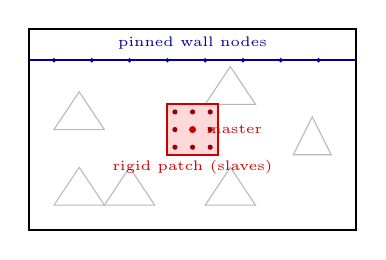
\begin{tikzpicture}[scale=0.80, every node/.style={font=\scriptsize}]
  \draw[thick] (-2.6,-1.6) -- (2.6,-1.6) -- (2.6,1.6) -- (-2.6,1.6) -- cycle;
  % triangulated mesh sketch
  \foreach \x/\y/\a/\b/\c/\d in {
    -2.2/-1.2/-1.4/-1.2/-1.8/-0.6,
    -1.4/-1.2/-0.6/-1.2/-1.0/-0.6,
    -2.2/-0.0/-1.4/-0.0/-1.8/0.6,
    0.2/-1.2/1.0/-1.2/0.6/-0.6,
    0.2/0.4/1.0/0.4/0.6/1.0,
    1.6/-0.4/2.2/-0.4/1.9/0.2
  } {\draw[gray!55] (\x,\y) -- (\a,\b) -- (\c,\d) -- cycle;}
  % column and rigid patch region
  \fill[red!15] (-0.4,-0.4) rectangle (0.4,0.4);
  \draw[red!80!black,thick] (-0.4,-0.4) rectangle (0.4,0.4);
  \filldraw[red!80!black] (0,0) circle (1.3pt);
  \node[red!80!black, right=1pt] at (0.02,0) {\tiny master};
  \foreach \p in {(-0.28,-0.28),(0.28,-0.28),(-0.28,0.28),(0.28,0.28),(0,-0.28),(0.28,0),(0,0.28),(-0.28,0)}
    \filldraw[red!60!black] \p circle (0.9pt);
  \node[red!80!black, font=\tiny] at (0, -0.6) {rigid patch (slaves)};
  % wall
  \draw[blue!60!black, thick] (-2.6,1.1) -- (2.6,1.1);
  \foreach \x in {-2.2,-1.6,-1.0,-0.4,0.2,0.8,1.4,2.0}
    \filldraw[blue!60!black] (\x,1.1) circle (0.7pt);
  \node[blue!60!black, font=\tiny, above] at (0,1.12) {pinned wall nodes};
\end{tikzpicture}
\vspace{-8pt}
\end{wrapfigure}

Boundary rings (outer $+$ holes) are densified to a target edge $h^{\!*}$, then fed to a constrained Delaunay triangulation (poly2tri). Steiner points are added as: (i) each column's (nudged) centroid, (ii) an $0.8\!\times$ footprint ring to populate the rigid patch, (iii) a wider $1.5\!\times$ ring for local refinement, (iv) wall samples at spacing $h^{\!*}$, (v) an interior grid at $1.5h^{\!*}$.

Centroids are iteratively nudged $\ge 0.5h^{\!*}$ away from every boundary segment so poly2tri does not reject them as collinear. The target edge is capped by
\[
h^{\!*}\;\le\;\min_{i}\bigl(\min(c_{1,i},c_{2,i})\bigr)\big/ 2,
\qquad
h^{\!*}\;\ge\;\max\!\bigl(d,\;L/32\bigr)
\]
so every column footprint contains $\gtrsim 4$ mesh nodes --- the condition for a well-posed rigid patch. If triangulation fails on any Steiner tier the solver retries with progressively stripped seeds (refine ring $\to$ tight ring $\to$ centroids only).

\section*{Element and assembly}
The DKT element enforces $\kappa = B\,u^e$ with the usual Specht/Batoz shape functions. Element stiffness is $k^e = \int_{A_e} B^{\!\top} D_b B\,dA$ with bending constitutive
\[
D_b = \frac{E h^3}{12(1-\nu^2)}\begin{bmatrix}1 & \nu & 0 \\ \nu & 1 & 0 \\ 0 & 0 & \tfrac{1-\nu}{2}\end{bmatrix},
\qquad
\kappa = \bigl(-w_{,xx},\,-w_{,yy},\,-2w_{,xy}\bigr)^{\!\top}.
\]
Elements assemble into sparse $K$ (CSR). Distributed load $q_u = (1.2\,w_D + 1.6\,w_L)/144$ psi is integrated against the translational shape functions to form $F$.

\section*{Boundary conditions}
Each column contributes (a) a \textbf{point pin} $w = 0$ at the master node, (b) rotational springs $k_{\theta x}, k_{\theta y}$ from the column's far-end fixity and length $H$, with $k_\theta = \alpha E_c I / H$, $\alpha\in[3,4]$, and (c) a \textbf{rigid master--slave patch} across all mesh nodes falling inside $c_1\!\times\! c_2$:
\[
w_s = w_m - dy\,\theta_{x,m} + dx\,\theta_{y,m},\quad
\theta_{x,s}=\theta_{x,m},\quad \theta_{y,s}=\theta_{y,m},
\]
where $(dx,dy)$ is the slave offset from the master. Slave rows/cols are folded into master rows and eliminated. The patch removes the plate singularity a point pin otherwise produces in DKT, giving mesh-independent $\theta$ at the column. Walls pin $w$ at every node within a half-target-edge of the wall segment.

\section*{Solve and recovery}
The reduced system $K_r u_r = F_r$ is solved with diagonal-preconditioned \textbf{conjugate gradients} to a residual tolerance $10^{-10}$. Per column:
\[
V_u \;=\; F[w\text{-DOF}] - (K u)[w\text{-DOF}],\quad
M_{u,2} = k_{\theta x}\,\theta_{x,m},\quad
M_{u,3} = k_{\theta y}\,\theta_{y,m}.
\]
$V_u$ and $M_u$ then feed the ACI 318 \S8.4 punching check ($b_0$, $\gamma_f$, $\gamma_v$, $v_c$). Equilibrium is audited: the total transferred reaction (column reactions $+$ wall reactions) must match the applied load to within $0.1\%$, flagged in the SolverPanel. A road-map upgrade replaces the node-reaction $M_u$ with a design-strip moment integration that is mesh-independent by construction and matches CSI SAFE methodology.

\end{document}
